\subsection{States of an Input Control}

\emph{Input controls} are Views receiving input from the user. The following state diagram 
explains the possible basic states of the underlying \emph{InputViewModel}:

% Graphic for TeX using PGF
% Title: P:\Kistl\Documentation\KistlGuide\Programming\Diagrams\InputStates.dia
% Creator: Dia v0.97.1
% CreationDate: Fri Mar 25 15:00:47 2011
% For: david
% \usepackage{tikz}
% The following commands are not supported in PSTricks at present
% We define them conditionally, so when they are implemented,
% this pgf file will use them.
\ifx\du\undefined
  \newlength{\du}
\fi
\setlength{\du}{15\unitlength}
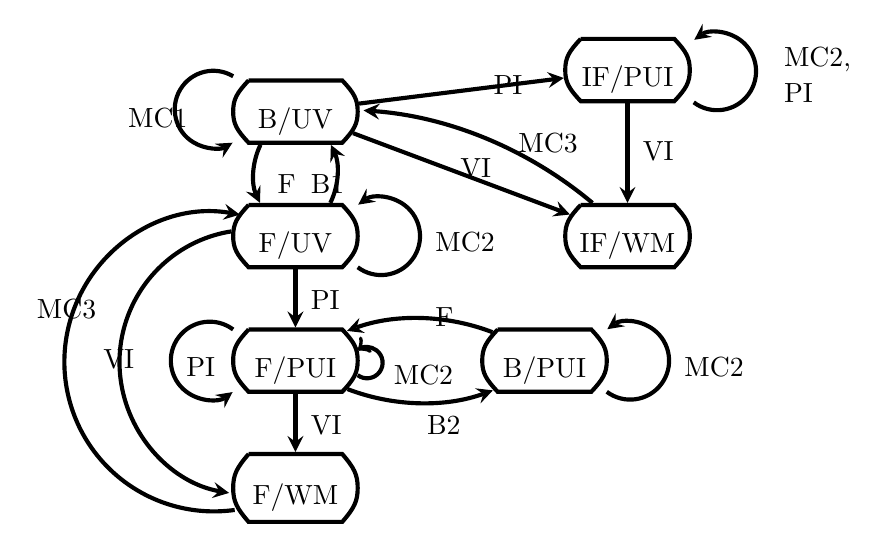
\begin{tikzpicture}
\pgftransformxscale{1.000000}
\pgftransformyscale{-1.000000}
\definecolor{dialinecolor}{rgb}{0.000000, 0.000000, 0.000000}
\pgfsetstrokecolor{dialinecolor}
\definecolor{dialinecolor}{rgb}{1.000000, 1.000000, 1.000000}
\pgfsetfillcolor{dialinecolor}
\pgfsetlinewidth{0.100000\du}
\pgfsetdash{}{0pt}
\pgfsetdash{}{0pt}
\pgfsetbuttcap
\pgfsetmiterjoin
\pgfsetlinewidth{0.100000\du}
\pgfsetbuttcap
\pgfsetmiterjoin
\pgfsetdash{}{0pt}
\definecolor{dialinecolor}{rgb}{1.000000, 1.000000, 1.000000}
\pgfsetfillcolor{dialinecolor}
\pgfpathmoveto{\pgfpoint{8.372180\du}{2.500000\du}}
\pgfpathlineto{\pgfpoint{10.627820\du}{2.500000\du}}
\pgfpathcurveto{\pgfpoint{10.909774\du}{2.800000\du}}{\pgfpoint{11.000000\du}{2.950000\du}}{\pgfpoint{11.000000\du}{3.250000\du}}
\pgfpathcurveto{\pgfpoint{11.000000\du}{3.550000\du}}{\pgfpoint{10.909774\du}{3.700000\du}}{\pgfpoint{10.627820\du}{4.000000\du}}
\pgfpathlineto{\pgfpoint{8.372180\du}{4.000000\du}}
\pgfpathcurveto{\pgfpoint{8.090226\du}{3.700000\du}}{\pgfpoint{8.000000\du}{3.550000\du}}{\pgfpoint{8.000000\du}{3.250000\du}}
\pgfpathcurveto{\pgfpoint{8.000000\du}{2.950000\du}}{\pgfpoint{8.090226\du}{2.800000\du}}{\pgfpoint{8.372180\du}{2.500000\du}}
\pgfusepath{fill}
\definecolor{dialinecolor}{rgb}{0.000000, 0.000000, 0.000000}
\pgfsetstrokecolor{dialinecolor}
\pgfpathmoveto{\pgfpoint{8.372180\du}{2.500000\du}}
\pgfpathlineto{\pgfpoint{10.627820\du}{2.500000\du}}
\pgfpathcurveto{\pgfpoint{10.909774\du}{2.800000\du}}{\pgfpoint{11.000000\du}{2.950000\du}}{\pgfpoint{11.000000\du}{3.250000\du}}
\pgfpathcurveto{\pgfpoint{11.000000\du}{3.550000\du}}{\pgfpoint{10.909774\du}{3.700000\du}}{\pgfpoint{10.627820\du}{4.000000\du}}
\pgfpathlineto{\pgfpoint{8.372180\du}{4.000000\du}}
\pgfpathcurveto{\pgfpoint{8.090226\du}{3.700000\du}}{\pgfpoint{8.000000\du}{3.550000\du}}{\pgfpoint{8.000000\du}{3.250000\du}}
\pgfpathcurveto{\pgfpoint{8.000000\du}{2.950000\du}}{\pgfpoint{8.090226\du}{2.800000\du}}{\pgfpoint{8.372180\du}{2.500000\du}}
\pgfusepath{stroke}
% setfont left to latex
\definecolor{dialinecolor}{rgb}{0.000000, 0.000000, 0.000000}
\pgfsetstrokecolor{dialinecolor}
\node at (9.500000\du,3.490000\du){B/UV};
\pgfsetlinewidth{0.100000\du}
\pgfsetdash{}{0pt}
\pgfsetdash{}{0pt}
\pgfsetbuttcap
\pgfsetmiterjoin
\pgfsetlinewidth{0.100000\du}
\pgfsetbuttcap
\pgfsetmiterjoin
\pgfsetdash{}{0pt}
\definecolor{dialinecolor}{rgb}{1.000000, 1.000000, 1.000000}
\pgfsetfillcolor{dialinecolor}
\pgfpathmoveto{\pgfpoint{8.372180\du}{5.500000\du}}
\pgfpathlineto{\pgfpoint{10.627820\du}{5.500000\du}}
\pgfpathcurveto{\pgfpoint{10.909774\du}{5.800000\du}}{\pgfpoint{11.000000\du}{5.950000\du}}{\pgfpoint{11.000000\du}{6.250000\du}}
\pgfpathcurveto{\pgfpoint{11.000000\du}{6.550000\du}}{\pgfpoint{10.909774\du}{6.700000\du}}{\pgfpoint{10.627820\du}{7.000000\du}}
\pgfpathlineto{\pgfpoint{8.372180\du}{7.000000\du}}
\pgfpathcurveto{\pgfpoint{8.090226\du}{6.700000\du}}{\pgfpoint{8.000000\du}{6.550000\du}}{\pgfpoint{8.000000\du}{6.250000\du}}
\pgfpathcurveto{\pgfpoint{8.000000\du}{5.950000\du}}{\pgfpoint{8.090226\du}{5.800000\du}}{\pgfpoint{8.372180\du}{5.500000\du}}
\pgfusepath{fill}
\definecolor{dialinecolor}{rgb}{0.000000, 0.000000, 0.000000}
\pgfsetstrokecolor{dialinecolor}
\pgfpathmoveto{\pgfpoint{8.372180\du}{5.500000\du}}
\pgfpathlineto{\pgfpoint{10.627820\du}{5.500000\du}}
\pgfpathcurveto{\pgfpoint{10.909774\du}{5.800000\du}}{\pgfpoint{11.000000\du}{5.950000\du}}{\pgfpoint{11.000000\du}{6.250000\du}}
\pgfpathcurveto{\pgfpoint{11.000000\du}{6.550000\du}}{\pgfpoint{10.909774\du}{6.700000\du}}{\pgfpoint{10.627820\du}{7.000000\du}}
\pgfpathlineto{\pgfpoint{8.372180\du}{7.000000\du}}
\pgfpathcurveto{\pgfpoint{8.090226\du}{6.700000\du}}{\pgfpoint{8.000000\du}{6.550000\du}}{\pgfpoint{8.000000\du}{6.250000\du}}
\pgfpathcurveto{\pgfpoint{8.000000\du}{5.950000\du}}{\pgfpoint{8.090226\du}{5.800000\du}}{\pgfpoint{8.372180\du}{5.500000\du}}
\pgfusepath{stroke}
% setfont left to latex
\definecolor{dialinecolor}{rgb}{0.000000, 0.000000, 0.000000}
\pgfsetstrokecolor{dialinecolor}
\node at (9.500000\du,6.490000\du){F/UV};
\pgfsetlinewidth{0.100000\du}
\pgfsetdash{}{0pt}
\pgfsetdash{}{0pt}
\pgfsetbuttcap
\pgfsetmiterjoin
\pgfsetlinewidth{0.100000\du}
\pgfsetbuttcap
\pgfsetmiterjoin
\pgfsetdash{}{0pt}
\definecolor{dialinecolor}{rgb}{1.000000, 1.000000, 1.000000}
\pgfsetfillcolor{dialinecolor}
\pgfpathmoveto{\pgfpoint{8.372180\du}{8.500000\du}}
\pgfpathlineto{\pgfpoint{10.627820\du}{8.500000\du}}
\pgfpathcurveto{\pgfpoint{10.909774\du}{8.800000\du}}{\pgfpoint{11.000000\du}{8.950000\du}}{\pgfpoint{11.000000\du}{9.250000\du}}
\pgfpathcurveto{\pgfpoint{11.000000\du}{9.550000\du}}{\pgfpoint{10.909774\du}{9.700000\du}}{\pgfpoint{10.627820\du}{10.000000\du}}
\pgfpathlineto{\pgfpoint{8.372180\du}{10.000000\du}}
\pgfpathcurveto{\pgfpoint{8.090226\du}{9.700000\du}}{\pgfpoint{8.000000\du}{9.550000\du}}{\pgfpoint{8.000000\du}{9.250000\du}}
\pgfpathcurveto{\pgfpoint{8.000000\du}{8.950000\du}}{\pgfpoint{8.090226\du}{8.800000\du}}{\pgfpoint{8.372180\du}{8.500000\du}}
\pgfusepath{fill}
\definecolor{dialinecolor}{rgb}{0.000000, 0.000000, 0.000000}
\pgfsetstrokecolor{dialinecolor}
\pgfpathmoveto{\pgfpoint{8.372180\du}{8.500000\du}}
\pgfpathlineto{\pgfpoint{10.627820\du}{8.500000\du}}
\pgfpathcurveto{\pgfpoint{10.909774\du}{8.800000\du}}{\pgfpoint{11.000000\du}{8.950000\du}}{\pgfpoint{11.000000\du}{9.250000\du}}
\pgfpathcurveto{\pgfpoint{11.000000\du}{9.550000\du}}{\pgfpoint{10.909774\du}{9.700000\du}}{\pgfpoint{10.627820\du}{10.000000\du}}
\pgfpathlineto{\pgfpoint{8.372180\du}{10.000000\du}}
\pgfpathcurveto{\pgfpoint{8.090226\du}{9.700000\du}}{\pgfpoint{8.000000\du}{9.550000\du}}{\pgfpoint{8.000000\du}{9.250000\du}}
\pgfpathcurveto{\pgfpoint{8.000000\du}{8.950000\du}}{\pgfpoint{8.090226\du}{8.800000\du}}{\pgfpoint{8.372180\du}{8.500000\du}}
\pgfusepath{stroke}
% setfont left to latex
\definecolor{dialinecolor}{rgb}{0.000000, 0.000000, 0.000000}
\pgfsetstrokecolor{dialinecolor}
\node at (9.500000\du,9.490000\du){F/PUI};
\pgfsetlinewidth{0.100000\du}
\pgfsetdash{}{0pt}
\pgfsetdash{}{0pt}
\pgfsetbuttcap
\pgfsetmiterjoin
\pgfsetlinewidth{0.100000\du}
\pgfsetbuttcap
\pgfsetmiterjoin
\pgfsetdash{}{0pt}
\definecolor{dialinecolor}{rgb}{1.000000, 1.000000, 1.000000}
\pgfsetfillcolor{dialinecolor}
\pgfpathmoveto{\pgfpoint{8.372180\du}{11.500000\du}}
\pgfpathlineto{\pgfpoint{10.627820\du}{11.500000\du}}
\pgfpathcurveto{\pgfpoint{10.909774\du}{11.827000\du}}{\pgfpoint{11.000000\du}{11.990500\du}}{\pgfpoint{11.000000\du}{12.317500\du}}
\pgfpathcurveto{\pgfpoint{11.000000\du}{12.644500\du}}{\pgfpoint{10.909774\du}{12.808000\du}}{\pgfpoint{10.627820\du}{13.135000\du}}
\pgfpathlineto{\pgfpoint{8.372180\du}{13.135000\du}}
\pgfpathcurveto{\pgfpoint{8.090226\du}{12.808000\du}}{\pgfpoint{8.000000\du}{12.644500\du}}{\pgfpoint{8.000000\du}{12.317500\du}}
\pgfpathcurveto{\pgfpoint{8.000000\du}{11.990500\du}}{\pgfpoint{8.090226\du}{11.827000\du}}{\pgfpoint{8.372180\du}{11.500000\du}}
\pgfusepath{fill}
\definecolor{dialinecolor}{rgb}{0.000000, 0.000000, 0.000000}
\pgfsetstrokecolor{dialinecolor}
\pgfpathmoveto{\pgfpoint{8.372180\du}{11.500000\du}}
\pgfpathlineto{\pgfpoint{10.627820\du}{11.500000\du}}
\pgfpathcurveto{\pgfpoint{10.909774\du}{11.827000\du}}{\pgfpoint{11.000000\du}{11.990500\du}}{\pgfpoint{11.000000\du}{12.317500\du}}
\pgfpathcurveto{\pgfpoint{11.000000\du}{12.644500\du}}{\pgfpoint{10.909774\du}{12.808000\du}}{\pgfpoint{10.627820\du}{13.135000\du}}
\pgfpathlineto{\pgfpoint{8.372180\du}{13.135000\du}}
\pgfpathcurveto{\pgfpoint{8.090226\du}{12.808000\du}}{\pgfpoint{8.000000\du}{12.644500\du}}{\pgfpoint{8.000000\du}{12.317500\du}}
\pgfpathcurveto{\pgfpoint{8.000000\du}{11.990500\du}}{\pgfpoint{8.090226\du}{11.827000\du}}{\pgfpoint{8.372180\du}{11.500000\du}}
\pgfusepath{stroke}
% setfont left to latex
\definecolor{dialinecolor}{rgb}{0.000000, 0.000000, 0.000000}
\pgfsetstrokecolor{dialinecolor}
\node at (9.500000\du,12.557500\du){F/WM};
\pgfsetlinewidth{0.100000\du}
\pgfsetdash{}{0pt}
\pgfsetdash{}{0pt}
\pgfsetbuttcap
\pgfsetmiterjoin
\pgfsetlinewidth{0.100000\du}
\pgfsetbuttcap
\pgfsetmiterjoin
\pgfsetdash{}{0pt}
\definecolor{dialinecolor}{rgb}{1.000000, 1.000000, 1.000000}
\pgfsetfillcolor{dialinecolor}
\pgfpathmoveto{\pgfpoint{16.372180\du}{1.500000\du}}
\pgfpathlineto{\pgfpoint{18.627820\du}{1.500000\du}}
\pgfpathcurveto{\pgfpoint{18.909774\du}{1.800000\du}}{\pgfpoint{19.000000\du}{1.950000\du}}{\pgfpoint{19.000000\du}{2.250000\du}}
\pgfpathcurveto{\pgfpoint{19.000000\du}{2.550000\du}}{\pgfpoint{18.909774\du}{2.700000\du}}{\pgfpoint{18.627820\du}{3.000000\du}}
\pgfpathlineto{\pgfpoint{16.372180\du}{3.000000\du}}
\pgfpathcurveto{\pgfpoint{16.090226\du}{2.700000\du}}{\pgfpoint{16.000000\du}{2.550000\du}}{\pgfpoint{16.000000\du}{2.250000\du}}
\pgfpathcurveto{\pgfpoint{16.000000\du}{1.950000\du}}{\pgfpoint{16.090226\du}{1.800000\du}}{\pgfpoint{16.372180\du}{1.500000\du}}
\pgfusepath{fill}
\definecolor{dialinecolor}{rgb}{0.000000, 0.000000, 0.000000}
\pgfsetstrokecolor{dialinecolor}
\pgfpathmoveto{\pgfpoint{16.372180\du}{1.500000\du}}
\pgfpathlineto{\pgfpoint{18.627820\du}{1.500000\du}}
\pgfpathcurveto{\pgfpoint{18.909774\du}{1.800000\du}}{\pgfpoint{19.000000\du}{1.950000\du}}{\pgfpoint{19.000000\du}{2.250000\du}}
\pgfpathcurveto{\pgfpoint{19.000000\du}{2.550000\du}}{\pgfpoint{18.909774\du}{2.700000\du}}{\pgfpoint{18.627820\du}{3.000000\du}}
\pgfpathlineto{\pgfpoint{16.372180\du}{3.000000\du}}
\pgfpathcurveto{\pgfpoint{16.090226\du}{2.700000\du}}{\pgfpoint{16.000000\du}{2.550000\du}}{\pgfpoint{16.000000\du}{2.250000\du}}
\pgfpathcurveto{\pgfpoint{16.000000\du}{1.950000\du}}{\pgfpoint{16.090226\du}{1.800000\du}}{\pgfpoint{16.372180\du}{1.500000\du}}
\pgfusepath{stroke}
% setfont left to latex
\definecolor{dialinecolor}{rgb}{0.000000, 0.000000, 0.000000}
\pgfsetstrokecolor{dialinecolor}
\node at (17.500000\du,2.490000\du){IF/PUI};
\pgfsetlinewidth{0.100000\du}
\pgfsetdash{}{0pt}
\pgfsetdash{}{0pt}
\pgfsetbuttcap
\pgfsetmiterjoin
\pgfsetlinewidth{0.100000\du}
\pgfsetbuttcap
\pgfsetmiterjoin
\pgfsetdash{}{0pt}
\definecolor{dialinecolor}{rgb}{1.000000, 1.000000, 1.000000}
\pgfsetfillcolor{dialinecolor}
\pgfpathmoveto{\pgfpoint{16.372180\du}{5.500000\du}}
\pgfpathlineto{\pgfpoint{18.627820\du}{5.500000\du}}
\pgfpathcurveto{\pgfpoint{18.909774\du}{5.800000\du}}{\pgfpoint{19.000000\du}{5.950000\du}}{\pgfpoint{19.000000\du}{6.250000\du}}
\pgfpathcurveto{\pgfpoint{19.000000\du}{6.550000\du}}{\pgfpoint{18.909774\du}{6.700000\du}}{\pgfpoint{18.627820\du}{7.000000\du}}
\pgfpathlineto{\pgfpoint{16.372180\du}{7.000000\du}}
\pgfpathcurveto{\pgfpoint{16.090226\du}{6.700000\du}}{\pgfpoint{16.000000\du}{6.550000\du}}{\pgfpoint{16.000000\du}{6.250000\du}}
\pgfpathcurveto{\pgfpoint{16.000000\du}{5.950000\du}}{\pgfpoint{16.090226\du}{5.800000\du}}{\pgfpoint{16.372180\du}{5.500000\du}}
\pgfusepath{fill}
\definecolor{dialinecolor}{rgb}{0.000000, 0.000000, 0.000000}
\pgfsetstrokecolor{dialinecolor}
\pgfpathmoveto{\pgfpoint{16.372180\du}{5.500000\du}}
\pgfpathlineto{\pgfpoint{18.627820\du}{5.500000\du}}
\pgfpathcurveto{\pgfpoint{18.909774\du}{5.800000\du}}{\pgfpoint{19.000000\du}{5.950000\du}}{\pgfpoint{19.000000\du}{6.250000\du}}
\pgfpathcurveto{\pgfpoint{19.000000\du}{6.550000\du}}{\pgfpoint{18.909774\du}{6.700000\du}}{\pgfpoint{18.627820\du}{7.000000\du}}
\pgfpathlineto{\pgfpoint{16.372180\du}{7.000000\du}}
\pgfpathcurveto{\pgfpoint{16.090226\du}{6.700000\du}}{\pgfpoint{16.000000\du}{6.550000\du}}{\pgfpoint{16.000000\du}{6.250000\du}}
\pgfpathcurveto{\pgfpoint{16.000000\du}{5.950000\du}}{\pgfpoint{16.090226\du}{5.800000\du}}{\pgfpoint{16.372180\du}{5.500000\du}}
\pgfusepath{stroke}
% setfont left to latex
\definecolor{dialinecolor}{rgb}{0.000000, 0.000000, 0.000000}
\pgfsetstrokecolor{dialinecolor}
\node at (17.500000\du,6.490000\du){IF/WM};
\pgfsetlinewidth{0.100000\du}
\pgfsetdash{}{0pt}
\pgfsetdash{}{0pt}
\pgfsetbuttcap
\pgfsetmiterjoin
\pgfsetlinewidth{0.100000\du}
\pgfsetbuttcap
\pgfsetmiterjoin
\pgfsetdash{}{0pt}
\definecolor{dialinecolor}{rgb}{1.000000, 1.000000, 1.000000}
\pgfsetfillcolor{dialinecolor}
\pgfpathmoveto{\pgfpoint{14.372180\du}{8.500000\du}}
\pgfpathlineto{\pgfpoint{16.627820\du}{8.500000\du}}
\pgfpathcurveto{\pgfpoint{16.909774\du}{8.800000\du}}{\pgfpoint{17.000000\du}{8.950000\du}}{\pgfpoint{17.000000\du}{9.250000\du}}
\pgfpathcurveto{\pgfpoint{17.000000\du}{9.550000\du}}{\pgfpoint{16.909774\du}{9.700000\du}}{\pgfpoint{16.627820\du}{10.000000\du}}
\pgfpathlineto{\pgfpoint{14.372180\du}{10.000000\du}}
\pgfpathcurveto{\pgfpoint{14.090226\du}{9.700000\du}}{\pgfpoint{14.000000\du}{9.550000\du}}{\pgfpoint{14.000000\du}{9.250000\du}}
\pgfpathcurveto{\pgfpoint{14.000000\du}{8.950000\du}}{\pgfpoint{14.090226\du}{8.800000\du}}{\pgfpoint{14.372180\du}{8.500000\du}}
\pgfusepath{fill}
\definecolor{dialinecolor}{rgb}{0.000000, 0.000000, 0.000000}
\pgfsetstrokecolor{dialinecolor}
\pgfpathmoveto{\pgfpoint{14.372180\du}{8.500000\du}}
\pgfpathlineto{\pgfpoint{16.627820\du}{8.500000\du}}
\pgfpathcurveto{\pgfpoint{16.909774\du}{8.800000\du}}{\pgfpoint{17.000000\du}{8.950000\du}}{\pgfpoint{17.000000\du}{9.250000\du}}
\pgfpathcurveto{\pgfpoint{17.000000\du}{9.550000\du}}{\pgfpoint{16.909774\du}{9.700000\du}}{\pgfpoint{16.627820\du}{10.000000\du}}
\pgfpathlineto{\pgfpoint{14.372180\du}{10.000000\du}}
\pgfpathcurveto{\pgfpoint{14.090226\du}{9.700000\du}}{\pgfpoint{14.000000\du}{9.550000\du}}{\pgfpoint{14.000000\du}{9.250000\du}}
\pgfpathcurveto{\pgfpoint{14.000000\du}{8.950000\du}}{\pgfpoint{14.090226\du}{8.800000\du}}{\pgfpoint{14.372180\du}{8.500000\du}}
\pgfusepath{stroke}
% setfont left to latex
\definecolor{dialinecolor}{rgb}{0.000000, 0.000000, 0.000000}
\pgfsetstrokecolor{dialinecolor}
\node at (15.500000\du,9.490000\du){B/PUI};
\pgfsetlinewidth{0.100000\du}
\pgfsetdash{}{0pt}
\pgfsetdash{}{0pt}
\pgfsetbuttcap
{
\definecolor{dialinecolor}{rgb}{0.000000, 0.000000, 0.000000}
\pgfsetfillcolor{dialinecolor}
% was here!!!
\pgfsetarrowsend{stealth}
\definecolor{dialinecolor}{rgb}{0.000000, 0.000000, 0.000000}
\pgfsetstrokecolor{dialinecolor}
\pgfpathmoveto{\pgfpoint{8.658505\du}{4.049987\du}}
\pgfpatharc{206}{155}{1.625000\du and 1.625000\du}
\pgfusepath{stroke}
}
\pgfsetlinewidth{0.100000\du}
\pgfsetdash{}{0pt}
\pgfsetdash{}{0pt}
\pgfsetbuttcap
{
\definecolor{dialinecolor}{rgb}{0.000000, 0.000000, 0.000000}
\pgfsetfillcolor{dialinecolor}
% was here!!!
\pgfsetarrowsend{stealth}
\definecolor{dialinecolor}{rgb}{0.000000, 0.000000, 0.000000}
\pgfsetstrokecolor{dialinecolor}
\pgfpathmoveto{\pgfpoint{10.341458\du}{5.450090\du}}
\pgfpatharc{26}{-25}{1.625000\du and 1.625000\du}
\pgfusepath{stroke}
}
\pgfsetlinewidth{0.100000\du}
\pgfsetdash{}{0pt}
\pgfsetdash{}{0pt}
\pgfsetbuttcap
{
\definecolor{dialinecolor}{rgb}{0.000000, 0.000000, 0.000000}
\pgfsetfillcolor{dialinecolor}
% was here!!!
\pgfsetarrowsend{stealth}
\definecolor{dialinecolor}{rgb}{0.000000, 0.000000, 0.000000}
\pgfsetstrokecolor{dialinecolor}
\pgfpathmoveto{\pgfpoint{7.956810\du}{6.136170\du}}
\pgfpatharc{261}{100}{3.194179\du and 3.194179\du}
\pgfusepath{stroke}
}
\pgfsetlinewidth{0.100000\du}
\pgfsetdash{}{0pt}
\pgfsetdash{}{0pt}
\pgfsetbuttcap
{
\definecolor{dialinecolor}{rgb}{0.000000, 0.000000, 0.000000}
\pgfsetfillcolor{dialinecolor}
% was here!!!
\pgfsetarrowsend{stealth}
\definecolor{dialinecolor}{rgb}{0.000000, 0.000000, 0.000000}
\pgfsetstrokecolor{dialinecolor}
\draw (9.500000\du,7.050171\du)--(9.500000\du,8.449829\du);
}
\pgfsetlinewidth{0.100000\du}
\pgfsetdash{}{0pt}
\pgfsetdash{}{0pt}
\pgfsetbuttcap
{
\definecolor{dialinecolor}{rgb}{0.000000, 0.000000, 0.000000}
\pgfsetfillcolor{dialinecolor}
% was here!!!
\pgfsetarrowsend{stealth}
\definecolor{dialinecolor}{rgb}{0.000000, 0.000000, 0.000000}
\pgfsetstrokecolor{dialinecolor}
\draw (9.500000\du,10.050201\du)--(9.500000\du,11.449898\du);
}
\pgfsetlinewidth{0.100000\du}
\pgfsetdash{}{0pt}
\pgfsetdash{}{0pt}
\pgfsetbuttcap
{
\definecolor{dialinecolor}{rgb}{0.000000, 0.000000, 0.000000}
\pgfsetfillcolor{dialinecolor}
% was here!!!
\pgfsetarrowsend{stealth}
\definecolor{dialinecolor}{rgb}{0.000000, 0.000000, 0.000000}
\pgfsetstrokecolor{dialinecolor}
\pgfpathmoveto{\pgfpoint{10.754445\du}{9.935407\du}}
\pgfpatharc{111}{70}{5.000000\du and 5.000000\du}
\pgfusepath{stroke}
}
\pgfsetlinewidth{0.100000\du}
\pgfsetdash{}{0pt}
\pgfsetdash{}{0pt}
\pgfsetbuttcap
{
\definecolor{dialinecolor}{rgb}{0.000000, 0.000000, 0.000000}
\pgfsetfillcolor{dialinecolor}
% was here!!!
\pgfsetarrowsend{stealth}
\definecolor{dialinecolor}{rgb}{0.000000, 0.000000, 0.000000}
\pgfsetstrokecolor{dialinecolor}
\pgfpathmoveto{\pgfpoint{14.245308\du}{8.564501\du}}
\pgfpatharc{291}{250}{5.000000\du and 5.000000\du}
\pgfusepath{stroke}
}
\pgfsetlinewidth{0.100000\du}
\pgfsetdash{}{0pt}
\pgfsetdash{}{0pt}
\pgfsetbuttcap
{
\definecolor{dialinecolor}{rgb}{0.000000, 0.000000, 0.000000}
\pgfsetfillcolor{dialinecolor}
% was here!!!
\pgfsetarrowsend{stealth}
\definecolor{dialinecolor}{rgb}{0.000000, 0.000000, 0.000000}
\pgfsetstrokecolor{dialinecolor}
\pgfpathmoveto{\pgfpoint{8.000012\du}{8.500009\du}}
\pgfpatharc{307}{54}{0.937500\du and 0.937500\du}
\pgfusepath{stroke}
}
\pgfsetlinewidth{0.100000\du}
\pgfsetdash{}{0pt}
\pgfsetdash{}{0pt}
\pgfsetbuttcap
{
\definecolor{dialinecolor}{rgb}{0.000000, 0.000000, 0.000000}
\pgfsetfillcolor{dialinecolor}
% was here!!!
\pgfsetarrowsend{stealth}
\definecolor{dialinecolor}{rgb}{0.000000, 0.000000, 0.000000}
\pgfsetstrokecolor{dialinecolor}
\pgfpathmoveto{\pgfpoint{10.999949\du}{6.999962\du}}
\pgfpatharc{127}{-126}{0.937500\du and 0.937500\du}
\pgfusepath{stroke}
}
\pgfsetlinewidth{0.100000\du}
\pgfsetdash{}{0pt}
\pgfsetdash{}{0pt}
\pgfsetbuttcap
{
\definecolor{dialinecolor}{rgb}{0.000000, 0.000000, 0.000000}
\pgfsetfillcolor{dialinecolor}
% was here!!!
\pgfsetarrowsstart{stealth}
\definecolor{dialinecolor}{rgb}{0.000000, 0.000000, 0.000000}
\pgfsetstrokecolor{dialinecolor}
\pgfpathmoveto{\pgfpoint{8.161190\du}{5.732611\du}}
\pgfpatharc{280}{82}{3.601966\du and 3.601966\du}
\pgfusepath{stroke}
}
\pgfsetlinewidth{0.100000\du}
\pgfsetdash{}{0pt}
\pgfsetdash{}{0pt}
\pgfsetbuttcap
{
\definecolor{dialinecolor}{rgb}{0.000000, 0.000000, 0.000000}
\pgfsetfillcolor{dialinecolor}
% was here!!!
\pgfsetarrowsend{stealth}
\definecolor{dialinecolor}{rgb}{0.000000, 0.000000, 0.000000}
\pgfsetstrokecolor{dialinecolor}
\draw (11.033691\du,3.058289\du)--(15.966309\du,2.441711\du);
}
\pgfsetlinewidth{0.100000\du}
\pgfsetdash{}{0pt}
\pgfsetdash{}{0pt}
\pgfsetbuttcap
{
\definecolor{dialinecolor}{rgb}{0.000000, 0.000000, 0.000000}
\pgfsetfillcolor{dialinecolor}
% was here!!!
\pgfsetarrowsend{stealth}
\definecolor{dialinecolor}{rgb}{0.000000, 0.000000, 0.000000}
\pgfsetstrokecolor{dialinecolor}
\draw (10.887695\du,3.770386\du)--(16.112305\du,5.729614\du);
}
\pgfsetlinewidth{0.100000\du}
\pgfsetdash{}{0pt}
\pgfsetdash{}{0pt}
\pgfsetbuttcap
{
\definecolor{dialinecolor}{rgb}{0.000000, 0.000000, 0.000000}
\pgfsetfillcolor{dialinecolor}
% was here!!!
\pgfsetarrowsend{stealth}
\definecolor{dialinecolor}{rgb}{0.000000, 0.000000, 0.000000}
\pgfsetstrokecolor{dialinecolor}
\draw (17.500000\du,3.048828\du)--(17.500000\du,5.451172\du);
}
\pgfsetlinewidth{0.100000\du}
\pgfsetdash{}{0pt}
\pgfsetdash{}{0pt}
\pgfsetbuttcap
{
\definecolor{dialinecolor}{rgb}{0.000000, 0.000000, 0.000000}
\pgfsetfillcolor{dialinecolor}
% was here!!!
\pgfsetarrowsend{stealth}
\definecolor{dialinecolor}{rgb}{0.000000, 0.000000, 0.000000}
\pgfsetstrokecolor{dialinecolor}
\pgfpathmoveto{\pgfpoint{16.655560\du}{5.450287\du}}
\pgfpatharc{310}{274}{9.625000\du and 9.625000\du}
\pgfusepath{stroke}
}
% setfont left to latex
\definecolor{dialinecolor}{rgb}{0.000000, 0.000000, 0.000000}
\pgfsetstrokecolor{dialinecolor}
\node[anchor=west] at (21.000000\du,2.000000\du){MC2,};
% setfont left to latex
\definecolor{dialinecolor}{rgb}{0.000000, 0.000000, 0.000000}
\pgfsetstrokecolor{dialinecolor}
\node[anchor=west] at (21.000000\du,2.800000\du){PI};
% setfont left to latex
\definecolor{dialinecolor}{rgb}{0.000000, 0.000000, 0.000000}
\pgfsetstrokecolor{dialinecolor}
\node[anchor=west] at (17.600000\du,4.200000\du){VI};
% setfont left to latex
\definecolor{dialinecolor}{rgb}{0.000000, 0.000000, 0.000000}
\pgfsetstrokecolor{dialinecolor}
\node[anchor=west] at (14.000000\du,2.600000\du){PI};
% setfont left to latex
\definecolor{dialinecolor}{rgb}{0.000000, 0.000000, 0.000000}
\pgfsetstrokecolor{dialinecolor}
\node[anchor=west] at (14.600000\du,4.000000\du){MC3};
% setfont left to latex
\definecolor{dialinecolor}{rgb}{0.000000, 0.000000, 0.000000}
\pgfsetstrokecolor{dialinecolor}
\node[anchor=west] at (13.200000\du,4.600000\du){VI};
% setfont left to latex
\definecolor{dialinecolor}{rgb}{0.000000, 0.000000, 0.000000}
\pgfsetstrokecolor{dialinecolor}
\node[anchor=west] at (12.600000\du,8.200000\du){F};
% setfont left to latex
\definecolor{dialinecolor}{rgb}{0.000000, 0.000000, 0.000000}
\pgfsetstrokecolor{dialinecolor}
\node[anchor=west] at (12.400000\du,10.800000\du){B2};
% setfont left to latex
\definecolor{dialinecolor}{rgb}{0.000000, 0.000000, 0.000000}
\pgfsetstrokecolor{dialinecolor}
\node[anchor=west] at (6.600000\du,9.400000\du){PI};
% setfont left to latex
\definecolor{dialinecolor}{rgb}{0.000000, 0.000000, 0.000000}
\pgfsetstrokecolor{dialinecolor}
\node[anchor=west] at (9.600000\du,7.800000\du){PI};
% setfont left to latex
\definecolor{dialinecolor}{rgb}{0.000000, 0.000000, 0.000000}
\pgfsetstrokecolor{dialinecolor}
\node[anchor=west] at (12.600000\du,6.400000\du){MC2};
% setfont left to latex
\definecolor{dialinecolor}{rgb}{0.000000, 0.000000, 0.000000}
\pgfsetstrokecolor{dialinecolor}
\node[anchor=west] at (9.600000\du,10.800000\du){VI};
% setfont left to latex
\definecolor{dialinecolor}{rgb}{0.000000, 0.000000, 0.000000}
\pgfsetstrokecolor{dialinecolor}
\node[anchor=west] at (4.600000\du,9.200000\du){VI};
% setfont left to latex
\definecolor{dialinecolor}{rgb}{0.000000, 0.000000, 0.000000}
\pgfsetstrokecolor{dialinecolor}
\node[anchor=west] at (3.000000\du,8.000000\du){MC3};
% setfont left to latex
\definecolor{dialinecolor}{rgb}{0.000000, 0.000000, 0.000000}
\pgfsetstrokecolor{dialinecolor}
\node[anchor=west] at (8.800000\du,5.000000\du){F};
% setfont left to latex
\definecolor{dialinecolor}{rgb}{0.000000, 0.000000, 0.000000}
\pgfsetstrokecolor{dialinecolor}
\node[anchor=west] at (9.600000\du,5.000000\du){B1};
\pgfsetlinewidth{0.100000\du}
\pgfsetdash{}{0pt}
\pgfsetdash{}{0pt}
\pgfsetbuttcap
{
\definecolor{dialinecolor}{rgb}{0.000000, 0.000000, 0.000000}
\pgfsetfillcolor{dialinecolor}
% was here!!!
\pgfsetarrowsend{stealth}
\definecolor{dialinecolor}{rgb}{0.000000, 0.000000, 0.000000}
\pgfsetstrokecolor{dialinecolor}
\pgfpathmoveto{\pgfpoint{8.000014\du}{2.400008\du}}
\pgfpatharc{301}{60}{0.928571\du and 0.928571\du}
\pgfusepath{stroke}
}
% setfont left to latex
\definecolor{dialinecolor}{rgb}{0.000000, 0.000000, 0.000000}
\pgfsetstrokecolor{dialinecolor}
\node[anchor=west] at (5.200000\du,3.400000\du){MC1};
\pgfsetlinewidth{0.100000\du}
\pgfsetdash{}{0pt}
\pgfsetdash{}{0pt}
\pgfsetbuttcap
{
\definecolor{dialinecolor}{rgb}{0.000000, 0.000000, 0.000000}
\pgfsetfillcolor{dialinecolor}
% was here!!!
\pgfsetarrowsend{stealth}
\definecolor{dialinecolor}{rgb}{0.000000, 0.000000, 0.000000}
\pgfsetstrokecolor{dialinecolor}
\pgfpathmoveto{\pgfpoint{16.999949\du}{9.999962\du}}
\pgfpatharc{127}{-126}{0.937500\du and 0.937500\du}
\pgfusepath{stroke}
}
% setfont left to latex
\definecolor{dialinecolor}{rgb}{0.000000, 0.000000, 0.000000}
\pgfsetstrokecolor{dialinecolor}
\node[anchor=west] at (18.600000\du,9.400000\du){MC2};
\pgfsetlinewidth{0.100000\du}
\pgfsetdash{}{0pt}
\pgfsetdash{}{0pt}
\pgfsetbuttcap
{
\definecolor{dialinecolor}{rgb}{0.000000, 0.000000, 0.000000}
\pgfsetfillcolor{dialinecolor}
% was here!!!
\pgfsetarrowsend{to}
\definecolor{dialinecolor}{rgb}{0.000000, 0.000000, 0.000000}
\pgfsetstrokecolor{dialinecolor}
\pgfpathmoveto{\pgfpoint{10.999980\du}{9.599985\du}}
\pgfpatharc{127}{-126}{0.375000\du and 0.375000\du}
\pgfusepath{stroke}
}
% setfont left to latex
\definecolor{dialinecolor}{rgb}{0.000000, 0.000000, 0.000000}
\pgfsetstrokecolor{dialinecolor}
\node[anchor=west] at (11.600000\du,9.600000\du){MC2};
\pgfsetlinewidth{0.100000\du}
\pgfsetdash{}{0pt}
\pgfsetdash{}{0pt}
\pgfsetbuttcap
{
\definecolor{dialinecolor}{rgb}{0.000000, 0.000000, 0.000000}
\pgfsetfillcolor{dialinecolor}
% was here!!!
\pgfsetarrowsend{stealth}
\definecolor{dialinecolor}{rgb}{0.000000, 0.000000, 0.000000}
\pgfsetstrokecolor{dialinecolor}
\pgfpathmoveto{\pgfpoint{19.094949\du}{3.028572\du}}
\pgfpatharc{127}{-126}{0.937500\du and 0.937500\du}
\pgfusepath{stroke}
}
\end{tikzpicture}


An InputViewModel has two distinct dimensions along which it modifies its behaviour. One is 
whether or not it currently has the focus\footnote{usually the keyboard focus}. The other 
dimension is whether or not there are outstanding (partial) modifications to the Value.

\begin{description}
\item[B] {The ViewModel is \emph{blurred}. That is, it does not have the focus. User input will not
 reach the control.}
\item[F] {The ViewModel is \emph{focused}. That is, it has the focus. The control will be notified
 of the user's next input.}
\item[IF] {The ViewModel is \emph{implicitely focused}. This states is reached by signalling user
 input without first signalling a focusing event. It is a convenient shortcut for Toolkits which do
 not track the concept of focus. Since this state is unaware of the user's focus, it has to bubble
 changes to the canonically formatted Value immediately to the View, possibly disrupting the user's
 input.}

\item[UV] {The View should display the \emph{unmodified Value}. This is the common state when no input was received or all input was processed successfully.}
\item[PUI] {The View should display a \emph{partial user input}. If the user cannot input a valid value atomically, the ViewModel will enter this state to keep track of the partial value to add more input from the user until a valid value is formed.}
\item[WM] {The ViewModel is currently \emph{writing to the Model}. Change notifications from the Model in this state are generated by the writing ViewModel and thus must be ignored locally.}
\end{description}

There are several events that determine the actual state of the InputViewModel.

\begin{description}
\item[F] {The ViewModel receives \emph{Focus}.}
\item[B1] {The ViewModel looses \emph{Focus}. Since this signals the user loosing interest in 
further editing this Value, a change in the FormattedValue is signalled\footnote{If the user has not
modified the Value, this signalling could be optimized away. Since the canonical representation 
should always be on display unless the user is currently editing this is not deemed an issue at this
time.} to update the View to the canonical representation of the Value.}
\item[B2] {The ViewModel looses \emph{Focus}. Since the user has still a pending partial input, the 
ViewModel expects the user to return and continue editing.}
\item[MC1] {The Model is \emph{changed} by a third party. This might be due to changes from the business 
logic or via other ViewModels. In any case the View should be signalled to update its display to 
the new Value.}
\item[MC2] {The Model is \emph{changed} by a third party. The user is currently editing the Value, so 
changes there should be ignored. In most cases this constitutes a programming error, as no code 
should try to change values while the user is editing them.}
\item[MC3] {The Model is \emph{changed} by the ViewModel. The View should be signalled to update its 
display to the new Value. Since this is in reaction to user input, this might not display a 
canonicalized value}
\item[PI] {The user enters \emph{partial input}. The ViewModel will store this until the user
completes or aborts\footnote{Canceling is currently not supported} her edit.}
\item[VI] {The user enters \emph{complete input}. The ViewModel accepts the input as valid and will
proceed to write it back to the Model.}
\end{description}
